\chapter{Optimization}

This chapter covers the following ideas. 

% A list of objectives for the chapter
%\begin{enumerate}
%\item ...
%\end{enumerate}

\begin{enumerate}
\item Explain the properties of the gradient, its relation to level
  curves and level surfaces, and how it can be used to find
  directional derivatives.  
\item Find equations of tangent planes using the gradient and level
  surfaces. Use the derivative (tangent planes) to approximate
  functions, and use this in real world application problems.
\item Explain the second derivative test in terms of eigenvalues.
  Illustrate how eigenvalues and eigenvectors are used to optimize
  functions of several variables.
\item Use Lagrange multipliers to optimize a function subject to
  constraints.  Explain why Lagrange multipliers works by considering
  the gradients of the function and the constraint at a maximum.
\end{enumerate}


%%% Local Variables: 
%%% mode: latex
%%% TeX-master: "../multivariable-calculus"
%%% End: 
%$

\section{The Gradient}

%Attach:20061020-notes-gradient.mw


For a function $f\colon \mathbb{R}^n\to\mathbb{R}$ with one output, the
derivative $Df$ when written as a vector is called the gradient of $f$
and written $\nabla f$\footnote{The ``$\nabla$'' symbol is called a ``nabla''
  and represents the mathematical ``del'' operation.  The mathematical
  expression $\nabla f$ is often spoken ``del f''.  You can think of $\nabla$ as
  a derivative symbol: it takes in a function and outputs the vector
  derivative.  }. If $C$ is a level curve $c=f(x,y)$ of the function
$f(x,y)$, and $\vec r(t)=\langle x(t), y(t)\rangle$ is a parametrization of the
curve in the plane, then the composition $f(\vec r(t))$ equals the
constant $c$. The chain rule for derivatives then shows that $Df D\vec
r=0$, or $\nabla f \cdot \vec r'=0$ (note that the row vector $Df$ times the
column vector $D\vec r$ is the same as the dot product $Df \cdot D\vec
r$). This means that the gradient is orthogonal to the direction
vector of a tangent line to the level curve, i.e. the gradient is
normal to level curves. Similarly, the gradient of a function
$f(x,y,z)$ is normal to level surfaces.  The pictures below illustrate
this idea for several functions.  The first two pictures show both a
2D and 3D plot of the same function.  The next two pictures give
contour plots and gradient field plots of two functions. The last plot
is a 3D plot of several level surfaces.  The gradient vectors are
normal to the level surfaces.

\begin{center}
\renewcommand{\mywidth}{1.15in}
\begin{tabular}{cccc}
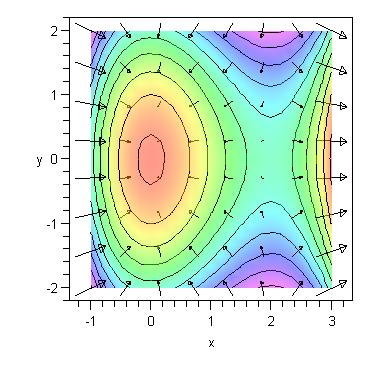
\includegraphics[width=\mywidth]{08-Optimization/support/levelcurve-1}
 
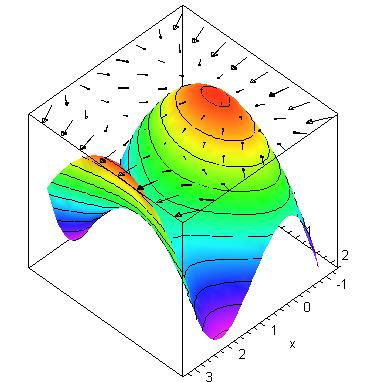
\includegraphics[width=\mywidth]{08-Optimization/support/levelcurve-2}&
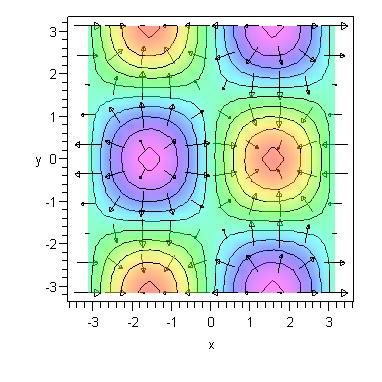
\includegraphics[width=\mywidth]{08-Optimization/support/levelcurve-3}&
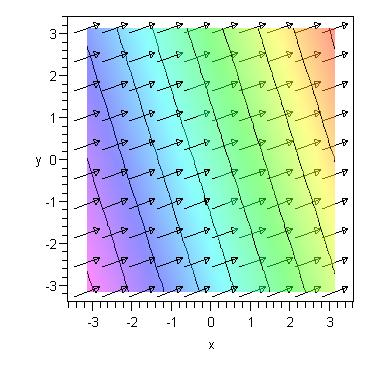
\includegraphics[width=\mywidth]{08-Optimization/support/levelcurve-4}&
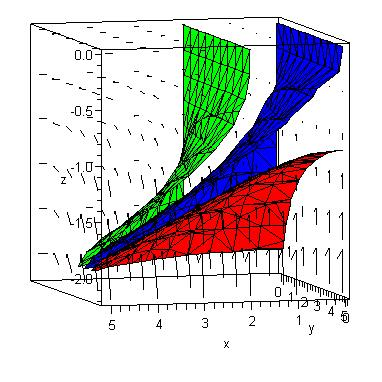
\includegraphics[width=\mywidth]{08-Optimization/support/levelsurface}\\
$f=x^3-3x^2-y^2+2$&
$f=\sin x\cos y$&
$f=3x+y$&
$f=x^2+yz^3$
\end{tabular}
\end{center}

\section{Directional derivatives}


For a function $z=f(x,y)$, the partial derivatives $f_x$ and $f_y$
give the slope of the function in the $x$ and $y$ directions,
respectively.  Furthermore, we know that the slope of the function is
zero in the directions that are orthogonal to the gradient at a point
from the previous sections.  Now we will calculate the slope of the
function in \emph{any} direction.

Let {$\vec u = \langle u_1,u_2\rangle$} be a unit vector
(representing any direction), and {$\vec p=(a,b)$} a point in the domain of
$f$. The directional derivative of $f$ in the direction of $\vec u$ at
the point $p=(a,b)$ is 
$$\ds D_{\vec u} f (\vec p) = \lim_{h\to
  0}\frac{f(\vec p + h\vec u) - f(\vec p)}{h}.$$ Geometrically, the
directional derivative is the slope of a tangent line to the surface
at $(a,b,f(a,b))$ which lies in a vertical plane containing the vector
$\langle u_1,u_2,0\rangle$ and the line $\vec q(t)=\langle a+u_1t,
b+u_2t\rangle$. The intersection of this vertical plane with the
surface is the space curve $\vec r(t) = \langle a+u_1t,b+u_2t,
f(a+u_1t,b+u_2t)\rangle=\langle a+u_1t, b+u_2t,f(\vec q(t))\rangle$,
which passes through the point $(a,b,f(a,b))$ at $t=0$.  The chain
rule gives the derivative of $\vec r$ at $t=0$ as $\vec r^\prime(0) =
\langle u_1,u_2,Df(\vec q(0))D\vec q(0)\rangle = \left<
  u_1,u_2,\begin{bmatrix}f_x(\vec p) & f_y(\vec
    p)\end{bmatrix}\begin{bmatrix}u_1\\u_2\end{bmatrix}\right> =
\langle u_1,u_2,\nabla f(\vec p)\cdot \vec u \rangle $. One unit
increase in the $\vec u$ direction gives a rise in the $z$ direction
of $\nabla f(a,b)\cdot \vec u$ units.  Hence we see that the
directional derivative is $$D_{\vec u} f (\vec p) = \nabla f(\vec
p)\cdot \vec u.$$ Since $\vec u$ is a unit vector, we can think of the
directional derivative in the direction $\vec u$ as the projection of
the gradient onto $\vec u$, i.e., $$D_{\vec u}f(\vec p) = \proj_{\vec
  u}\nabla f(\vec p).$$

Since $D_{\vec u} f (\vec p) = \nabla f(\vec p)\cdot \vec u = |\nabla
f(\vec p)||\vec u|\cos\theta$, where $\theta$ is the angle between
$\nabla f(\vec p)$ and $\vec u$, we see that the directional
derivative is greatest when $\cos\theta=1$, i.e., when $\theta =
0$. The direction of greatest increase is given by the gradient.  The
direction of greatest decrease is opposite the gradient, where
$\theta=\pi$.  The function does not increase or decrease (i.e., it
stays level) where $\theta=\pi/2,-\pi/2$.  In these directions are the
contour lines of the function.  In other words, the gradient is
orthogonal to the contour lines of the function.  This matches up with
what we saw previously.


Recall the differential notation $dy=f' dx$ from first-semester
calculus.  This can be extended to all dimensions as $d\vec y=D\vec f
d\vec x$, or $d(\text{outputs}) =Df d(\text{inputs})$. For a function
$z=f(x,y)$, we have
$dz=\begin{bmatrix}f_x&f_y\end{bmatrix}\begin{bmatrix}dx\\dy\end{bmatrix}$.
If $\vec u =\langle u_1,u_2\rangle$ is a unit vector, then a change in the inputs
$dx=u_1$ and $dy=u_2$ gives a change in the output $dz$ as the
directional derivative in the direction of $\vec u$. We again have
$D_{\vec u} f (\vec p) = D f(\vec p)\vec u = \nabla f(\vec p)\cdot \vec u$.
Interpretations about the gradient come immediately when you use the
differential notation $d(\text{outputs}) =Df d(\text{inputs})$.



\begin{example}
 \marginpartop{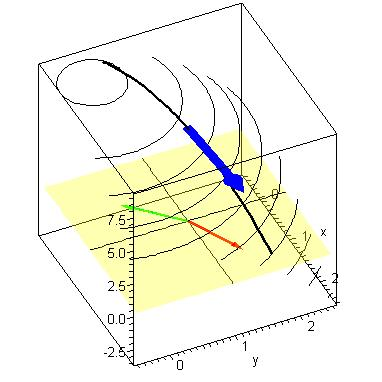
\includegraphics[width=\marginparwidth]{08-Optimization/support/dirder}}%
The function $f(x,y)=9-x^2-y^2$ has deriviative
$Df=\begin{bmatrix}-2x&-2y\end{bmatrix}$, i.e. $\nabla f = \langle-2x,-2y\rangle$ The
directional derivative in the $\vec u = \langle1,0\rangle$ direction at some point
point $(x,y)$ is $D_{\vec u}f(x,y)=\langle-2x,-2y\rangle\cdot\langle1,0\rangle=-2x$, or the
derivative in the $x$ direction.  The directional derivative in the
direction $\langle2,1\rangle$ (which as a unit vector is
$\frac{1}{\sqrt{5}}\langle2,1\rangle$) is
$D_{\langle2,1\rangle}f(x,y)=\langle-2x,-2y\rangle\cdot\frac{1}{\sqrt{5}}\langle2,1\rangle=\frac{1}{\sqrt{5}}(-4x-2y)$.
At the point $(1,1)$, we have $\nabla f(1,1) = \langle-2,-2\rangle$ and
$D_{\langle2,1\rangle}f(1,1)=\langle-2,-2\rangle\cdot \frac{1}{\sqrt 5}\langle2,1\rangle=-\frac{6}{\sqrt{5}}$.
The direction of greatest increase at $(1,1)$ is in the $\langle-2,-2\rangle$
direction. This is illustrated in the picture to the left. The $xy$
plane is shaded in the picture. The direction of the gradient points
back to the origin (it is a 2D vector).  The direction of $u$ points
away from the origin (hence the dot product is negative). Several
level curves of $f$ are drawn in 3D with their height included.  The
space curve shown is a curve in the surface. A tangent vector to that
curve is also drawn. The change in height of that tangent vector is
the directional derivative, as the change in the $xy$ direction is 1
unit.
\end{example}



\section{Tangent planes and Approximation}
Since the gradient is normal to level surfaces, the gradient $\nabla
f(x,y,z)$ of function $f(x,y,z)$ can be used to find the tangent plane
to level surfaces.  For example, the hyperboloid of one sheet
$1=x^2+y^2-z^2$ is the level surface $f=1$ of the function
$f=x^2+y^2-z^2$. The point $(1,-2,2)$ is on this hyperboloid, so the
gradient $\nabla f(x,y,z)=\langle2x,2y,-2z\rangle$ evaluated at $(1,-2,2)$ gives the
vector $\nabla f(1,-2,2)= \langle2,-4,-4\rangle$, which is a normal vector for the
tangent plane to the hyperboloid at $(1,-2,2)$.  An equation of the
tangent plane is thus $2(x-1)-4(y+2)-4(z-2)=0$. 

If a surface can be written in the form $z=f(x,y)$, then the function
$g(x,y,z) = z-f(x,y)$ has as its gradient $\nabla g = \langle-f_x,-f_y,1\rangle$.
Hence, a normal vector to the tangent plane of a surface $z=f(x,y)$ is
$\vec n = \langle-f_x,-f_y,1\rangle$, which we already discovered as $\vec n =
\langle1,0,f_x\rangle\times\langle0,1,f_y\rangle$.

The differential {$dy=f^\prime dx$} says a little change in {$y$} can be
approximated by multiplying the derivative by a little change in
{$x$}.  For a function $f\colon \mathbb{R}^n\to\mathbb{R}^m$, the
\textbf{differential} is $d\vec y = D\vec f d\vec x$, where $D\vec f$
is the derivative, {$d\vec y$} is an $m$ dimensional vector of changes
in the outputs, and {$d\vec x$} is an $n$ dimensional vector of
changes in the inputs. We estimate changes in our outputs by
multiplying the derivative by changes in our inputs.
For a function $z=f(x,y)$, this gives $dz=f_xdx+f_ydy$. If we write
our change in inputs as $\langle dx,dy\rangle = \vec u ds$ for a unit vector $\vec
u$ with magnitude $ds$, then a change in  $z$ is approximately $dz =
Df\vec u ds= D_{\vec u}f ds$, or the product of the directional
derivative and $ds$.

\note{Follow this order: think of the approximation as traveling a bit of distance along the directional vector (and do a problem as such).  Then think of it as $d\vec y=D\vec f d\vec x$, and work the same problem that way.}

The differential formula $d\vec y=D\vec f d\vec x$ can be used to
connect ideas about tangent lines, tangent planes, and approximation
in all dimensions.  The following table summarizes how to use this
notation in various settings.
\begin{center}
\begin{tabular}{|c|c|c|c|c|c|}
\hline
Function & $d\vec y$ & $Df$ & $d\vec x$ & $\vec x=\vec c$ & Tangent
space (line, plane, etc.)\\
 &  &  &  &  & $d\vec y = D\vec f(\vec c) d\vec x$\\
 &  &  &  &  & $\vec y - \vec f(\vec c) = D\vec f(\vec c) (\vec x-\vec
c)$\\\hline
$y=f(x)$ & $dy$ & $f^\prime$ & dx & $x=c$& $y - f(c) = f^\prime(c) ( x -
c)$\\\hline

$\vec r(t)=\langle x,y,z\rangle$ & $\begin{bmatrix}dx\\dy\\dz\end{bmatrix}$ &
$\begin{bmatrix}x^\prime(t)\\y^\prime(t)\\z^\prime(t)\end{bmatrix}$ & $dt$ & $t=c$& 
$\begin{bmatrix}x-x(c)\\y-y(c)\\z-z(c)\end{bmatrix} =
\begin{bmatrix}x^\prime(c)\\y^\prime(c)\\z^\prime(c)\end{bmatrix} ( t - c)$\\\hline

$z=f(x,y)$ & $dz$ & $\begin{bmatrix}f_x&f_y\end{bmatrix}$ &
$\begin{bmatrix}dx\\dy\end{bmatrix}$ & $(x,y)=(a,b)$ & $z-f(a,b) =
\begin{bmatrix}f_x(a,b)&f_y(a,b)\end{bmatrix}
\begin{bmatrix}x-a\\y-b\end{bmatrix}$\\\hline

$\vec r(u,v)=\langle x,y,z\rangle$ & $\begin{bmatrix}dx\\dy\\dz\end{bmatrix}$ 
& $\begin{bmatrix}x_u &x_v\\y_u&y_v\\z_u&z_v\end{bmatrix}$ 
& $\begin{bmatrix}du\\dv\end{bmatrix}$
& $(u,v)=(a,b)$& $
\begin{bmatrix}x-x(a,b)\\y-y(a,b)\\z-z(a,b)\end{bmatrix} =
\begin{bmatrix}x_u &x_v\\y_u&y_v\\z_u&z_v\end{bmatrix}
\begin{bmatrix}u-a\\v-b\end{bmatrix}$\\\hline

\end{tabular}
\end{center}
A change $d\vec y$ in output is the output variable $\vec y$ minus its
value $\vec f(\vec c)$ at the input $\vec c$. A change $d\vec x$ in
the input is the variable $\vec x$ minus its value at $\vec c$.
Tangent planes can be found in all dimensions using this notation.

\begin{example}
We can use differential notation to estimate changes in a function. If
the temperature at a point in the plane is given by
{$T(x,y)=x^2-xy-y^2$} degrees Fahrenheit, and a particle is at
{$(2,3)$}, estimate the change in temperature if the particle moves
about .1 units in the direction of {$\langle3,4\rangle$}. The gradient of $T$ is
$\nabla T = \langle2x-y,-x-2y\rangle$, which at $(2,3)$ is $\nabla T(2,3) = \langle1,-8\rangle$. The
change in inputs is $\langle dx,dy\rangle = .1\frac{\langle3,4\rangle}{|\langle3,4\rangle|} =
\frac{.1}{5}\langle3,4\rangle = \langle.06,.08\rangle$.  We calculate the change in
temperature (the output) as $dT = DT(2,3)
\begin{bmatrix}dx\\dy\end{bmatrix} = T_x dx+T_ydy = (1)(.06)+(-8)(.08)
= -.58$. So the temperature will decrease a little over half a degree.   
\end{example}

\begin{example}
A rectangle is rather wide and short.  When you measure the edges of
the rectangle to estimate the area, which edge must be measured more
precisely to not affect the area of the rectangle?  Area is
$A(h,w)=hw$, so $dA =
\begin{bmatrix}A_h&A_w\end{bmatrix}\begin{bmatrix}dh\\dw\end{bmatrix}
= \begin{bmatrix}w&h\end{bmatrix}\begin{bmatrix}dh\\dw\end{bmatrix} =
wdh+hdw$. Since $w$ is large, a small change $dh$ in the measurement
of the height will have a much larger affect on the change in area. 
Hence, you must be more precise when measuring the shorter height.
\end{example}

\begin{example}
The total resistance {$R$} in a circuit with two parallel resistors
with resistance {$R_1$} and {$R_2$} is given by the formula {$
\frac{1}{R} = \frac{1}{R_1}+\frac{1}{R_2} $}.  Solving for $R$ and
taking derivatives, one can show that {$ dR =
\begin{bmatrix}\frac{R^2}{R_1^2} & \frac{R^2}{R_2^2} \end{bmatrix}
\begin{bmatrix}dR_1\\dR_2\end{bmatrix}$}. If {$ R_1 $} changes from 10
to 9.9, and {$ R_2 $} changes from 20 to 20.2, would you expect a
positive or negative change in the total resistance {$R$}? We have
$dR_1 = -.1$ and $dR_2=.2$, and $\frac{1}{R} = \frac{3}{20},$ so
$R=20/3$ and $dR = \begin{bmatrix}\frac{(20/3)^2}{10^2} &
\frac{(20/3)^2}{20^2} \end{bmatrix}
\begin{bmatrix}-.1\\.2\end{bmatrix} = 
(2/3)^2(-.1) + (1/3)^2(.2) = -4/90+2/90=-2/90<0$ which is negative.
Manufactures of circuit boards have to account for variations in the
resistance of resistors.  Differentials allow them to estimate total
changes in resistance due to possible changes in each resistor. 
\end{example}

% \subsection{Local Linearization}
% The textbook discusses the ``Local linearization'' of a function as
% $L(x,y) = f(a,b) + f_x(a,b)(x-a)+f_y(a,b)(y-b)$, which is equivalent
% to $L(x,y)-f(a,b) = df$, or $L=f+dz$ (just add the function to the
% change in the function to get an approximate value for the function at
% $(x,y)$).  The error $dz = L(x,y)-f(a,b)$ in approximating $f$ is also
% called $E(x,y)$ in the book.  You can estimate how much error there is
% by the formula {$ |E|\leq\frac{1}{2}M(|dx|+|dy|)^2 $}, where $M$ is any
% upper bound for the values $|f_{xx}|,|f_{yy}|$, and $|f_{xy}|$. The
% value of this formula is that it tells you how far off the change $dz$
% could be from the real change $\Delta z = f(x+dx,y+dy)-f(x,y)$ in output.

\section{The Second Derivative Test}
If a function $y=f(x)$ has a relative extremum at $x=c$, then
$f^\prime(c)=0$ or the derivative is undefined. The places where the
derivative is either zero or undefined are called critical values of
the function. The first derivative test allows you to check the value
of the derivative on both sides of the critical value and then
interpret whether that point is a maximum or minimum using
increasing/decreasing arguments.  The second derivative test requires
you to compute the second derivative at $x=c$. If $f^{\prime\prime}(c)>0$ (the
function is concave upwards), then the function has a minimum at
$x=c$. If $f^{\prime\prime}(c)<0$ (the function is concave downwards), then the
function has a maximum at $x=c$. If $f^{\prime\prime}(c)=0$, then the second
derivative test fails.

The first derivative test breaks down in higher dimensions because
there are more than two ways to approach a point of the domain. All that
can be said is that at an extreme value, the gradient is zero (as the
tangent plane should be horizontal). In higher dimensions, there are
three classifications of critical points: maximum, minimum, saddle
point (a point where the tangent plane is horizontal, but in some
directions you increase and in other directions you decrease). The
second derivative test does not break down. To understand the second
derivative test, we need to learn about eigenvalues and eigenvectors
of a matrix.

If {$z=f(x,y)$}, then $Df(x,y) = \begin{bmatrix}f_x&f_y\end{bmatrix}$
is a vector field with two inputs and two outputs. Its derivative
{$D^2f (x,y)= \begin{bmatrix}f_{xx}&f_{xy}\\f_{yx}&f_{yy}\end{bmatrix}
  $} is a {$2\times 2$} square matrix called the Hessian of $f$. This
matrix is symmetric (i.e., $f_{xy}=f_{yx}$) if $f$ is twice
continuously differentiable.

An eigenvector is a vector (direction), such that multiplication by
the matrix is the same as multiplying the vector by a scalar (that
scalar is called an eigenvalue). Notationally this is written {$ A\vec
v=\lambda \vec v $}, where {$ \lambda $} is the eigenvalue and $\vec v$ is an
eigenvector. Eigenvalues can be found by subtracting {$\lambda$} from each
of the entries on the diagonal of a square matrix, and then asking for
which values of {$\lambda$} the determinant equals zero (solve {$ \det(A-\lambda I)
= 0 $}). In linear algebra, you will learn much more about
eigenvectors and eigenvalues. For example, the eigenvalues of the
matrix {$ \begin{bmatrix}2&1 \\1&2\end{bmatrix} $} are found as
follows. Write {$ \det \begin{bmatrix}2-\lambda&1 \\1&2-\lambda\end{bmatrix} =0$}.
Compute the determinant and set it equal to zero: {$(2-\lambda)(2-\lambda)-(1)(1) = 0$} or {$4-4\lambda + \lambda^2 -1 = 0$}. Hence
{$\lambda^2-4\lambda +3 = (\lambda-3)(\lambda -1) = 0$} or the eigenvalues are {$\lambda = 1,3$}. 

Another way to find eigenvalues follows from some linear algebra
theorems that we won't prove.  First, for a square matrix, the
determinant is the product of the eigenvalues.  Second, the sum of
diagonal elements (the \emph{trace} of the matrix) is the sum of the
eigenvalues.  This makes it easy to solve for the eigenvalues of a $2\times
2$ matrix.  For the example above, the determinant of $
\begin{bmatrix}
  2&1\\1&2
\end{bmatrix}$ is $4-1=3$ and the trace is $4$.  We need to find two
numbers such that the product is 3 and the sum is 4.  That is, $xy=3$
and $x+y=4$.  You may have already guessed that the values are $1$ and
$3$.  Therefore, $x=4-y$, so $(4-y)y=3$, so $y^2-4y-3=0$.  Solving
this for $y$ gives $y=1,3$.  Substituting and solving for $x$ then
gives us $x=3,1$, respectively.  In either case, we see that the
eigenvalues are $1$ and $3$.


%The notation {$D^2f$} for {$y=f(x)$} gives a {$1\times 1$} matrix
% $[f^{\prime\prime}(x)]$. The eigenvalue of this matrix is $f^{\prime\prime}(x)$. The
% second derivative test checks to see if that eigenvalue is positive or
% negative at a critical value.
%\begin{enumerate}
%	\item If the eigenvalue is positive at a critical point$x=c$,
% then the function is concave upwards and we have found a minimum.
%  \item If the eigenvalue is negative at a critical point$x=c$, then
% the function is concave downwards and we have found a maximum.
%\end{enumerate}

The eigenvalues of $D^2f$ give the ``directional'' second derivative
in the direction of a corresponding eigenvector. The largest
eigenvalue is the largest possible value of the second derivative in
any direction. The smallest eigenvalue is the smallest possible value
of the second derivative in any direction. The \textbf{second
derivative test} follows: If the eigenvalues are all positive at a
critical point, then in every direction the function is concave
upwards, which means that the function has a minimum at that critical
point.  If all the eigenvalues are negative, then in every direction
the function is concave downwards, and function has a maximum there. 
If there is a positive eigenvalue and a negative eigenvalue, the
function has a saddle point there.  If either the largest or smallest
eigenvalue is zero, then the second derivative test fails. 

%In higher dimensions, the second derivative test requires that we
% first locate all critical values $(a,b)$ where the gradient of {$f$}
% is the zero vector. Then find the eigenvalues of {$D^2f(a,b)$} (notice
% that you have to evaluate the derivative at the critical point). One
% of the following 4 options occurs.
%\begin{enumerate}
%	\item If all the eigenvalues are positive, then in every
% direction the function {$f$} is concave upwards, which means that you
% have found a minimum at $(a,b)$.
%	\item If all the eigenvalues are negative, then in every
% direction the function {$f$} is concave downwards, which means that
% you have found a maximum at $(a,b)$.
%	\item If some eigenvalues are positive and some are negative,
% then you have found a saddle point at $(a,b)$.
%	\item If either the largest eigenvalue or smallest eigenvalue
% is zero, then the second derivative test fails.
%\end{enumerate}

%
%For the function {$f(x,y)=x^2+4x+y^2-2y$}, the gradient is $Df =
% \begin{bmatrix}2x+4&2y-2 \end{bmatrix}$, which is zero at $x=-2,y=1$.
% The Hessian is $D^2f = \begin{bmatrix}2&0 \\0&2\end{bmatrix}$. The
% eigenvalues are found by solving $0=\det \begin{bmatrix}2-\lambda &0 \\0&2-\lambda
% \end{bmatrix} = (2-\lambda)^2$, so $\lambda =2$ is a double root.  Since all the
% eigenvalues are positive, the function is concave up in every
% direction at $(-2,1)$, which means that $f(-2,1)=-5$ is a minimum
% value of $f$. 


\begin{example} 
  For the function {$f(x,y)=x^2-6xy+y^2$}, the gradient is $Df =
  \begin{bmatrix}2x-6y&-6x+2y \end{bmatrix}$, which is zero only at
  $x=0,y=0$ (solve the system of equations $2x-6y=0,-6x+2y=0$). The
  Hessian is $D^2f = \begin{bmatrix}2&-6 \\-6&2\end{bmatrix}$. The
  eigenvalues are found by solving $0=\det \begin{bmatrix}2-\lambda
    &-6 \\-6&2-\lambda \end{bmatrix} = (2-\lambda)^2-36 =
  4-4\lambda+\lambda^2 -36 = (\lambda-8)(\lambda+4)$, so $\lambda =
  8,-4$ are the eigenvalues.  Since there is a positive eigenvalue and
  a negative eigenvalue, the function is concave upwards in one
  direction and concave downwards in another direction, so there is a
  saddle point at the origin.
\end{example}

\begin{example}
  For the function {$f(x,y)=x^3-3x+y^2-4y$}, the gradient is $Df =
  \begin{bmatrix}3x^2-3&2y-4 \end{bmatrix}$, which is zero at
  $x=1,y=2$ or $x=-1,y=2$. Hence there are two critical points. The
  Hessian is $D^2f = \begin{bmatrix}6x&0 \\0&2\end{bmatrix}$. Since
  there are two critical points, we have to find the eigenvalues of
  two matrices.  When $x=-1,y=2$, the eigenvalues of
  $\begin{bmatrix}-6&0 \\0&2\end{bmatrix}$ are $\lambda=-6,2$. Since
  one is positive and one is negative, there is a saddle point at
  $(-1,2)$. When $x=1,y=2$, the eigenvalues of $\begin{bmatrix}6&0
    \\0&2\end{bmatrix}$ are $\lambda=6,2$.  Since both are positive,
  there is a minimum at $(-1,2)$ (as in every direction the function
  is concave upwards).
\end{example}

\begin{example}
  We can use these ideas to find the dimensions of the rectangular
  prism of maximum volume that is located above the {$xy$} plane, and
  below the paraboloid {$z=9-x^2-y^2$}. We want to maximize the
  function $V(x,y) = (2x)(2y)(9-x^2-y^2)$.  The gradient is zero at
  $x=3/2,y=3/2$, and the Hessian at that critical point is
  $\begin{bmatrix}-54&-18 \\-18&-54\end{bmatrix}$. The eigenvalues are
  $\lambda = -36,-72$, which are both negative, which means we have
  found a maximum. I skipped a lot of details which you can check. The
  maximum volume is $f(3/2,3/2)=81/2$ and occurs at $(3/2,3/2)$. Since
  $x$ is only half the length, the dimensions are $3$ by $3$ by $9/2$.
\end{example}

If the domain of a function is restricted to a small region, then you
use the second derivative test to find the optimum solutions on the
interior of the domain.  You use the first derivative test on the
boundary of the domain to find the optimum solutions on the boundary.
If a function is continuous on a domain that is closed (includes its
boundary) and bounded, then there will always be a maximum and minimum
(this is called the extreme value theorem).


\section{Lagrange Multipliers}

To optimize a function {$f$}, subject to a constraint (such as a
height restriction, or a budget constraint for a business), we use a
technique called Lagrange Multipliers. Let {$f$} be the function you
want to optimize and {$g = 0$} be the constraint. Define $L=f-\lambda
g$ for some scalar lambda which will be determined. Find where all
partial derivatives of {$L$} are zero.  Under suitable conditions, the
optimum solutions will be a solution of $\nabla L=\vec 0$.  In other
words, the optimum solutions will be a solution of the equations
$\nabla f = \lambda \nabla g$ and $g==0$.

\begin{example}
  To find the dimensions of the rectangular prism of maximum volume
  that is located above the {$xy$} plane, and below the paraboloid
  {$z=9-x^2-y^2$}, we want to optimize the volume function
  $f(x,y,z)=4xyz$.  Our constraint is the height of $z$, which we
  rewrite as $g(x,y,z)=z-(9-x^2-y^2)=0$.  The Lagrangian is
  $L(x,y,z,\lambda)=4xyz - \lambda(z-9+x^2+y^2)$, and so the partials
  of $L$ are $L_x = 4yz-2\lambda x, L_y=4xz-2\lambda y,
  L_z=4xy-\lambda, L_\lambda = -(z-9+x^2+y^2)$. We now set each
  partial equal to zero and solve the system of equations.  We solve
  the first three equations for $\lambda$ to obtain $\lambda =
  \frac{4yz}{2x} = \frac{4xz}{2y}= \frac{4xy}{1}$.  The equation
  $\frac{4yz}{2x} = \frac{4xz}{2y}$ means $y^2=x^2$ or $x=y$ as the
  values for $x$ and $y$ must both be positive.  The equation
  $\frac{4xz}{2y}= \frac{4xy}{1}$ means $4z=8y^2$ or $z=2y^2$.  The we
  now substitute $x=y$ and $z=2y^2$ into the equation
  $L_\lambda=-g(x,y,z)=0=-(z-9+x^2+y^2)$ to obtain $2y^2-9+y^2+y^2=0$
  or $y^2=9/4$ so $y=3/2$.  Hence $x=3/2,z=9/2$ and the dimensions are
  $3$ by $3$ by $9/2$.
\end{example}

\begin{example}
  To find the point closest to the origin on the hyperbolic cylinder
  {$x^2-z^2=1$}, we want to optimize the distance
  $f=\sqrt{x^2+y^2+z^2}$ subject to the constraint
  $g=x^2-z^2-1=0$. However, the square root in the optimization
  function will result in rather messy derivatives, so instead we
  notice that distance is minimized at the same places where distance
  squared is minimized, so we can use $f=x^2+y^2+z^2$ instead.  The
  Lagrangian is $L=x^2+y^2+z^2-\lambda(x^2-z^2-1)$. The gradient is
  $\nabla L(x,y,z,\lambda) = \langle2x-2\lambda x, 2y, 2z+2\lambda x,
  -(x^2-z^2-1)\rangle$. We now solve for when the gradient is zero to
  obtain $2x-2\lambda x = 2x(1-\lambda)=0, 2y=0, 2z(1+\lambda)=0$ for
  the first three equations.  From the first equation we have $x=0$ or
  $\lambda=1$. However the constraint $x^2-z^2=1$ (which is
  $L_\lambda=0$) shows that $x\neq 0$, which means that $\lambda=1$.
  The second partial tells us that $y=0$, and the third partial shows
  us that $2z(2)=0$ or $z=0$.  Since $z=0$, we have using our
  constraint again that $x=\pm 1$. So there are two solutions
  $(-1,0,0)$ and $(1,0,0)$.
\end{example}



\subsection{Why Lagrange Multipliers works - linear dependence}
If the domains of {$f$} and the constraint $g$ are 2 dimensional, then
{$g=0$} represents a level curve of the function {$g$}. At a maximum
of {$f$} where {$g=0$}, the level curve of {$f$} which passes through
the location of the maximum will have a tangent line that is parallel
to the level curve of {$g$}.  Hence, the gradients of {$f$} and {$g$}
should be parallel, as they are normal to level curves (and since they
are normal to the same tangent line, they should be parallel). Hence
the gradient of {$f$} is a scalar multiple of the gradient of {$g$}. 
Call that scalar {$\lambda$}.  Then {$\nabla f=\lambda\nabla g$}. Hence, at a maximum or
minimum we will have {$0=\nabla f-\lambda\nabla g$}.  This is equivalent to solving 
{$\nabla L =\vec 0$}.


If the domains of {$f$} and the constraint are 3 dimensional, then
{$g=0$} represents a level surface of the function {$g$}. At a maximum
of {$f$} where {$g=0$}, the level surface of {$f$} which passes
through the location of the maximum will have a tangent plane that is
tangent to the level surface {$g=0$}.  Hence, the gradients of {$f$}
and {$g$} should be parallel as they are both normal vectors to the
same tangent plane.  So the gradient of {$f$} is a scalar multiple of
the gradient of {$g$}.  This line of reasoning extends to all
dimensions.


If you have multiple constraints, then let the Lagrangian be
{$L=f-\lambda_1g_1-\lambda_2g_2-\cdots$}. Under suitable conditions,
it can be shown that optimum solutions will satisfy the equation
{$\nabla L = 0$}. Just keep subtracting a new variable times the next
constraint for each new constraint. This works precisely because at an
optimal solution, it can be shown that the gradient of $f$ is a linear
combination of the gradients of the constraints, i.e. $\nabla f =
\lambda_1g_1+\cdots +\nabla_ng_n$. You will learn more about this
topic when you study linear algebra.

\section{Taylor Series}
Recall that a Taylor series centered at $x=a$ for a function $f(x)$ is
$\sum_{n=0}^{\infty}\frac{f^{(n)}(a)}{n!}(x-a)^n$.  This formula holds as well
for arbitrary functions if you replace $f^{(n)}(a)$ with the linear
transformation $D^n\vec f(\vec a)$ and write $\sum_{n=0}^{\infty}\frac{D^n\vec
  f(\vec a)}{n!}(\vec x-\vec a)^n$. However, interpreting this formula
requires knowledge about linear transformations, and becomes rather
messy to write in matrix notation. Quadratic forms appear as the
degree two term of the Taylor series.  You can use the Taylor series
to prove the second derivative test.  Further information can be found
by consulting the free textbook written by Kenneth Kuttler at BYU
Provo (though be warned that it is written for an advanced student).
For this book, see
\url{http://www.math.byu.edu/~klkuttle/calcbookB.pdf}.






%%% Local Variables: 
%%% mode: latex
%%% TeX-master: "../multivariable-calculus"
%%% End: 





